%!TeX root = main.tex
%!encoding = UTF-8 Unicode

\subsection{Probe Architecture and Implementation}
\label{sec:design_voltage}
This section presents the design and implementation of the dual-channel differential active voltage probe (DAVP). The probe implements the methods introduced in Chapter~\ref{ch:Methods} and meets the requirements defined in Section~\ref{sec:VoltageRequirements}.

\begin{figure}[ht]
	\centering
	\import{./figures/4_VoltageProbe/}{Diss_SchematicOverviewEMEProbe.pdf_tex}
	\caption{Schematic overview of DAVP functionality.}\label{fig:OverviewEMEProbe}
\end{figure}


The functional architecture is shown in \fref{fig:OverviewEMEProbe}, and the implemented hardware is shown in \fref{fig:Pic_EMEProbe}. 
The design comprises three main blocks: a frequency-compensated voltage divider, a unity-gain stage, and two subtractor paths. The following sections describe the purpose and design of each block, together with the relevant implementation choices and measured performance.

\begin{figure}[ht]
	\centering
	\import{./figures/4_VoltageProbe/}{Diss_Pic_EMEv5c.pdf_tex}
	\caption{Photograph of redesigned dual-channel differential active voltage probe.}\label{fig:Pic_EMEProbe}
\end{figure}

\FloatBarrier







\subsubsection*{Frequency-Compensated Voltage Divider}
The frequency-compensated voltage divider is the probe's input stage. It attenuates the drain-source voltage of the MOSFET to a level suitable for the subsequent amplifiers while maintaining a flat frequency response over the target bandwidth.

The divider is particularly sensitive to parasitic effects because its high impedance makes even small parasitic capacitances produce significant time constants. At the same time, the physical dimensions must be kept small to satisfy the transmission-line length constraint and limit parasitic inductance. 


\begin{table}
	\caption{Parameter values of frequency compensated voltage divider}
	\label{tab:VoltageDividerParameters}
	\centering
	\begin{tabular}{lll}
		\toprule
		\textbf{Parameter} & \textbf{Symbol} & \textbf{Value} \\
		\midrule
		High-voltage resistor &\mi{R}{HV} & \SI{2}{M\Omega} \\
		Sense resistor &\mi{R}{sens} & \SI{2.5}{k\Omega} \\
		Sense capacitor &\mi{C}{sens} & \SI{156}{pF} \\
		High-voltage capacitor &\mi{C}{HV} & \SI{0.2}{pF} \\
		\bottomrule
	\end{tabular}
\end{table}



At low frequencies, the divider ratio is determined by the resistors. 
At higher frequencies, parasitic capacitances of the resistors and PCB form a capacitive divider whose ratio generally differs from the resistive ratio, resulting in a non-flat frequency response. 
To form a frequency-compensated voltage divider, capacitors larger than the parasitic capacitances are connected in parallel with the resistors and adjusted so that the effective capacitive and resistive divider ratios match:

\begin{equation}
	\mi{a}{CR} = \frac{\mi{R}{sens}}{\mi{R}{sens} + \mi{R}{HV}} = \frac{\mi{C}{HV,tot}}{\mi{C}{sens} + \mi{C}{HV,tot}}.
	\label{eq:divider_ratio}
\end{equation}
Here, $\mi{C}{HV,tot} = \mi{C}{HV} + \mi{C}{\sigma 1,HV}$ includes both the implemented high-voltage capacitor and the parallel parasitic capacitance of the high-voltage resistor. 
Additionally, the high-voltage resistor is split into two equivalent series resistors $\mi{R}{HV} = \mi{R}{HV1} + \mi{R}{HV2}$.
The equivalent circuit in \fref{fig:VoltageDividerPCB_parESB} shows these contributions together with the other parasitic elements considered in the divider design.

\begin{figure}[ht]
	\centering
	\import{./figures/4_VoltageProbe/}{Diss_VoltageDividerPCB_parESB.pdf_tex}
	\caption{Equivalent circuit of the frequency-compensated voltage divider including the relevant parasitic elements.}\label{fig:VoltageDividerPCB_parESB}
\end{figure}

The divider ratio is chosen to use the full input range of the subsequent unity-gain stage.
The required attenuation follows from the maximum probe input voltage and the allowable input voltage of this stage.
A probe input of \SI{1200}{V} must therefore be attenuated to approximately \SI{2.6}{V}, corresponding to $\mi{a}{CR} = 1/460$.
The component selection described below must achieve this ratio despite the limited availability of parts suitable for both high-voltage and high-frequency operation.

\paragraph*{Sense Capacitor {\boldmath\mi{C}{sens}}:}
The sense capacitor must provide the required capacitance while maintaining a self-resonance frequency above the probe's target bandwidth. This frequency is given by
\begin{equation}
	\mi{f}{res} = \frac{1}{2\pi\sqrt{\mi{C}{sens}\cdot\mi{L}{\sigma,sens}}}.
\end{equation}
Commercially available capacitor technologies intended for high-frequency use were evaluated using a VNA within the probe's voltage-divider and unity-gain circuit rather than as standalone components.
Port 1 was connected to the high-impedance input of the voltage divider, and port 2 to the output of the unity-gain stage.
The unity-gain stage provides a \SI{50}{\Omega} output impedance.
Its bandwidth exceeds the capacitor resonance frequencies considered here, as shown in \fref{fig:VNA_rawUG} and discussed below.
Compared with a direct one-port measurement of the capacitor, this two-port arrangement reduces the influence of de-embedding errors on the estimated parasitic inductance.
The in-circuit measurements therefore provide the basis for the following comparison of capacitor technologies.

\begin{figure}[ht]
	\centering
	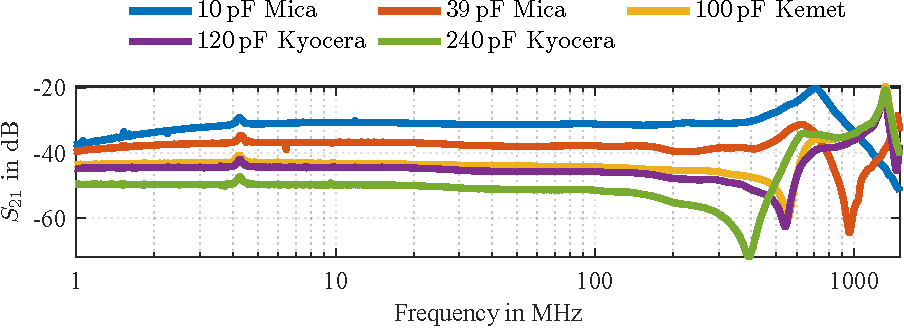
\includegraphics[scale=1]{figures/4_VoltageProbe/Voltage_Csense_Comp.pdf}
	\caption{Comparison of different sense capacitor technologies.}\label{fig:CapacitorComparison}
\end{figure}

\fref{fig:CapacitorComparison} shows the measured forward transmission $\mi{S}{21}$ for each evaluated sense capacitor.
Differences in the transmission magnitude reflect the different capacitance values.
The resonance peaks, in contrast, arise from the interaction of the capacitance and parasitic inductance.
The inductance was therefore estimated from the measured capacitance and resonance frequency using the resonance relation given above.
The resulting inductance estimates in \tref{tab:CapComp} lie between approximately \SI{680}{pH} and \SI{820}{pH}.
All evaluated capacitors use the same standard 0805 package.
The similar inductances therefore suggest that package size, rather than capacitor technology, is the dominant factor.

\begin{table}[ht]
	\caption{Comparison of different high-frequency capacitor technologies.}
	\label{tab:CapComp}
	\centering
	\begin{tabular}{l l l l l}
		\toprule
		Manufacturer & Technology & Capacitance & Resonance Frequency & Calc. Inductance\\
		\midrule
		{Illinois} {Capacitor} & Mica & \SI{10}{pF} & -- & -- \\
		{Illinois} {Capacitor} & Mica & \SI{39}{pF} & \SI{956}{MHz} & \SI{710}{pH} \\
		Kemet & MLCC & \SI{100}{pF} & \SI{555}{MHz} & \SI{822}{pH} \\
		Kyocera & MLCC & \SI{120}{pF} & \SI{540}{MHz} & \SI{723}{pH} \\
		Kyocera & MLCC & \SI{240}{pF} & \SI{393}{MHz} & \SI{683}{pH} \\
		\bottomrule
	\end{tabular}
\end{table}

The similar package inductances require a sufficiently small capacitance per capacitor to keep the resonance frequency above the target bandwidth of \SI{500}{MHz}.
Increasing the capacitance of a single capacitor would lower its resonance frequency if the package inductance remained unchanged.
The total sense capacitance can nevertheless be increased by connecting several of these small-capacitance capacitors in parallel.
For identical capacitors, the total capacitance ideally increases in proportion to the number of capacitors, while the equivalent parasitic inductance decreases by the same factor.
Therefore, the resonance frequency should remain unchanged.
The practical effectiveness of this approach was evaluated using parallel-connected \SI{39}{pF} mica capacitors, as shown in \fref{fig:CsenseParallel}.

\begin{figure}[ht]
	\centering
	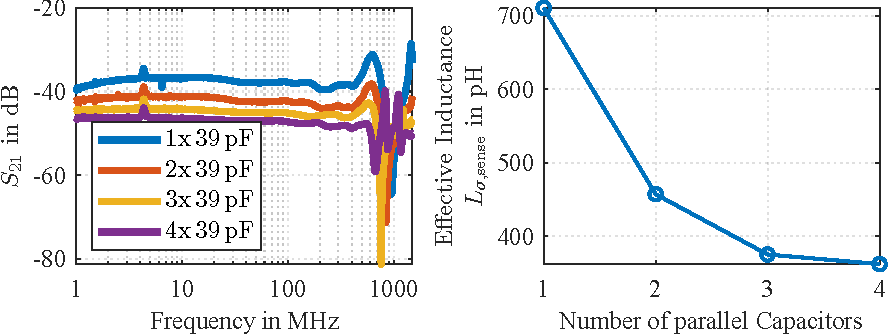
\includegraphics[scale=1]{figures/4_VoltageProbe/Voltage_Csense_parallel.pdf}
	\caption{Behavior of parallel-connected sense mica capacitors.}\label{fig:CsenseParallel}
\end{figure}

The measured resonance frequency decreases as more capacitors are added because the PCB interconnects contribute additional inductance. 
For four parallel capacitors, the calculated equivalent parasitic inductance decreases by a factor of only 1.9 relative to a single capacitor, rather than the ideal factor of four. 
Nevertheless, up to four capacitors can be connected in parallel while keeping the resonance frequency above the target bandwidth. 
The selected four-capacitor configuration provides a total capacitance of \SI{156}{pF} and a resonance frequency of \SI{670}{MHz}.


\FloatBarrier

\paragraph*{High-Voltage Capacitor {\boldmath\mi{C}{HV}}:}
With the sense capacitance fixed, the required high-voltage capacitance follows from the divider ratio in \eref{eq:divider_ratio}.
The parasitic capacitance \mi{C}{\sigma 1,HV} of the high-voltage resistor contributes to this value, as shown in \fref{fig:VoltageDividerPCB_parESB}.
The additional capacitance required is therefore
\begin{equation}
	\mi{C}{HV} = \frac{\mi{a}{CR}}{1-\mi{a}{CR}} \cdot \mi{C}{sens} - \mi{C}{\sigma 1,HV}.
\end{equation}
This value defines the capacitance to be implemented in each signal path.

The high-voltage capacitor \mi{C}{HV} was implemented as a PCB-integrated parallel-plate capacitor because no available discrete capacitor technology meets both the high-voltage and high-frequency requirements.
Integration avoids a separate component package and its mounting connections.
Removing these elements can reduce the associated parasitic inductance.
The electrode geometry and connecting traces must nevertheless remain compact to limit inductive effects at high frequencies.

The capacitors in the two signal paths are arranged symmetrically to help maintain matched capacitive-divider ratios.
\fref{fig:VoltageDividerPCB} shows the electrode arrangement in a cross-section of the probe PCB.
The positive signal path uses copper areas on the top and second PCB layers.
The negative signal path uses the corresponding bottom and fifth layers.
A mismatch in the capacitive-divider ratios would convert part of a common-mode input into a differential signal.
Matching the two ratios is therefore necessary to preserve the probe's CMRR at high frequencies.

\begin{figure}[ht]
	\centering
	\import{./figures/4_VoltageProbe/}{Diss_VoltageDividerPCB_3D.pdf_tex}
	\caption{Cross-section of the redesigned dual-channel differential active voltage probe PCB.}\label{fig:VoltageDividerPCB}
\end{figure}

For a given PCB dielectric and layer spacing, the electrode overlap area determines the nominal capacitance.
The area required for the calculated value of \mi{C}{HV} is estimated using the parallel-plate relation
\begin{equation}
	\mi{C}{HV} = \frac{\varepsilon_0 \cdot \varepsilon_r \cdot A}{d},
\end{equation}
where $A$ is the overlapping electrode area, $d$ is the dielectric thickness, and $\varepsilon_r$ is its relative permittivity.
This calculation provides a nominal electrode area that must allow for subsequent adjustment to compensate for component and manufacturing tolerances.

The electrode overlap area is adjustable to compensate for variations in the capacitance.
Both the resistor's parasitic capacitance and the PCB prepreg thickness are subject to significant tolerances.
\fref{fig:VoltageDividerPCB_Polygon} shows the finger layout used to make the overlap area adjustable.
The active overlap area is selected using \SI{0}{\Omega} resistors to adjust the divider ratio.
The divider ratio is adjusted iteratively using VNA measurements until the target value is achieved.

\begin{figure}[ht]
	\centering
	\import{./figures/4_VoltageProbe/}{Diss_VoltageDividerPCB_Polygons.pdf_tex}
	\caption{Finger layout of the trimmable PCB capacitor.}\label{fig:VoltageDividerPCB_Polygon}
\end{figure}


\paragraph*{Resistor Selection {\boldmath\mi{R}{HV} \& \mi{R}{sens}}}
The resistor values primarily determine the divider's low-frequency behavior, whereas its intended high-frequency response is governed by the capacitive elements.
At low frequencies, \mi{R}{HV} and \mi{R}{sens} set the divider ratio according to \eref{eq:divider_ratio}.
The $RC$ time constant formed by \mi{R}{HV} and the implemented high-voltage capacitance \mi{C}{HV} gives the characteristic frequency at which the capacitive behavior starts to dominate.
\begin{align}	
	\mi{f}{c} &= \frac{1}{2\pi \cdot \mi{R}{HV} \cdot \mi{C}{HV}} \\
				&= \frac{1}{2\pi \cdot \SI{2}{M\Omega} \cdot \SI{0.2}{pF}} \approx \SI{400}{kHz}.
\end{align}
Although the intended response is predominantly capacitive well above this frequency, resistor parasitics can still affect the high-frequency behavior.

The high-voltage resistance is limited to \SI{2}{M\Omega} to reduce the influence of parasitic capacitance on the high-frequency response.
Problems occured with the parasitic capacitance \mi{C}{\sigma 2,HV}, which forms between the resistor's conductive path and the sense polygon.
Together with the resistance, this capacitance introduces time constants that can affect the frequency range of interest.
The selected resistance is therefore lower than the \SI{10}{M\Omega} commonly used in commercial high-voltage probes.
A thin-film rather than a thick-film resistor is used to further reduce the parasitic effect.
\fref{fig:VoltageDividerPCB_Polygon} also shows the PCB cutout beneath the resistor, which reduces capacitive coupling to the sense polygon.
The resistance, resistor technology, and PCB geometry are thus selected together to limit the influence of this parasitic capacitance.

\paragraph*{Shielding}
Shielding is used to reduce capacitive coupling between the positive and negative signal paths.
In the earlier four-layer PCB, parasitic capacitance \mi{C}{\sigma 2,sens} coupled the two paths.
\fref{fig:VoltageDividerPCB} shows the shielding layer introduced between the paths in the redesigned six-layer PCB.
This layer reduces the interchannel coupling identified in the earlier design.











\FloatBarrier

\subsubsection*{Unity-Gain Amplifier}
A unity-gain stage buffers the voltage divider to isolate it from the loading introduced by the subsequent subtractor circuits.
The divider's output impedance varies with frequency because of the sense capacitance.
The buffer must therefore combine high input impedance with a low, approximately constant output impedance.
Low noise and sufficient bandwidth are required to preserve the switching waveform for analyses such as overshoot, \sddt{v}, and \mi{e}{sw}, while also enabling accurate high-frequency measurement.
These requirements motivate an architecture that combines DC precision with wide bandwidth.

A composite-loop architecture was selected to combine the complementary characteristics of a precision operational amplifier and a high-speed buffer.
Precision operational amplifiers provide low offset and drift but have limited gain-bandwidth products.
High-speed buffers, in contrast, offer multi-gigahertz bandwidth and high slew rates but typically have poorer DC and input impedance characteristics.
The composite loop assigns low- and high-frequency signal components to separate paths so that each amplifier contributes in its intended frequency range.

\fref{fig:EME_ESB_UG} shows the composite-loop circuit used to implement the two signal paths.
The series capacitor \mi{C}{2} and resistor \mi{R}{3} form a high-pass filter at the input of the high-speed buffer \mti{OP}{1}.
This network directs high-frequency signal components to the feedforward path with buffer gain $G$.
The precision operational amplifier \mti{OP}{2} processes the low-frequency path and drives the buffer's auxiliary input to control the output voltage \mi{v}{UG}.
The two paths thus provide high-frequency transmission and low-frequency correction within the same stage.
\tref{tab:UG_Parameters} lists the component values used in this implementation.

\begin{figure}[ht]
	\centering
	\import{./figures/4_VoltageProbe/}{Diss_UnityGain_EME_ESB.pdf_tex}
	\caption{Equivalent circuit diagram of the unity-gain stage, which is designed as a composite loop amplifier.}\label{fig:EME_ESB_UG}
\end{figure}

\begin{table}[ht]
	\caption{Parameter values of the unity-gain amplifier}\label{tab:UG_Parameters}
	\centering
	\begin{tabular}[t]{l l}
		\toprule
		\textbf{Parameter} & \textbf{Value}\\
		\midrule
		\mti{OP}{1} & BUF802 			\\
		\mi{R}{1} & \SI{52.2}{k\Omega}	\\
		\mi{R}{3} & \SI{30}{\Omega}		\\		
		\mi{R}{5} & \SI{10}{k\Omega}	\\
		\mi{R}{8} & \SI{10}{\Omega}		\\
		\mi{C}{1} & n.p. 				\\
		\mi{C}{3} & \SI{27}{pF}			\\
		\bottomrule
	\end{tabular}
	\hspace{1cm}
	\begin{tabular}[t]{l l}
		\toprule
		\textbf{Parameter} & \textbf{Value}\\
		\midrule
		\mti{OP}{2} & OPA140 \\
		\mi{R}{2} & \SI{11}{k\Omega} \\
		\mi{R}{4} & \SI{2.44}{k\Omega} \\
		\mi{R}{6} & \SI{2}{k\Omega} \\
		\mi{R}{9} & \SI{80}{k\Omega}\\
		\mi{C}{2}  & \SI{270}{pF} \\
		\mi{C}{4} & \SI{100}{pF} \\
		\bottomrule
	\end{tabular}
\end{table}

The low- and high-frequency path gains must match to obtain a flat response through the crossover region.
The low-frequency gain is set by the input attenuation factor $\alpha$ and the feedback factor $\beta$ of the precision-amplifier path.
According to the buffer datasheet, matching this gain to the buffer gain $G$ requires
\begin{align}
	\sfrac{\alpha}{\beta} &= G \\
	\alpha &= \frac{\mi{R}{2}}{\mi{R}{1} + \mi{R}{2}}  \\
	\beta &= \frac{\mi{R}{4}}{\mi{R}{4} + \mi{R}{5}}
\end{align}
Because $G$ varies between devices, the precision amplifier's feedback network must be trimmed during commissioning to satisfy this matching condition.

In addition to matching the paths within each amplifier, the positive and negative unity-gain stages must have equal overall gains.
Device-to-device gain variations and unequal loading by the subtractor can cause an interchannel gain mismatch.
A voltage divider formed by \mi{R}{8} and \mi{R}{9} is therefore trimmed during commissioning to balance the two channels.
Any residual mismatch converts a common-mode input into a non-zero differential output and degrades the CMRR.

\fref{fig:VNA_rawUG} shows the small-signal frequency response of the unity-gain stage measured using a VNA.
The magnitude of $\mi{S}{21}$ is approximately \SI{-2.2}{dB} at low frequencies and exhibits a small peak of approximately \SI{-1.6}{dB} near \SI{3.6}{MHz}.
Relative to the low-frequency transmission level, the measured \SI{3}{dB} bandwidth is approximately \SI{320}{MHz}.
Above this frequency, the transmission decreases gradually, reaching approximately \SI{-11.7}{dB} at \SI{1}{GHz}.
The bandwidth therefore identifies a relative attenuation level rather than a sharp upper limit of transmission.

The isolated unity-gain stage was measured with its input configured for a nominal impedance of \SI{50}{\Omega}.
The measured input reflection coefficient $\mi{S}{11}$ indicates that the input was not perfectly matched to the VNA reference impedance.
Input mismatch must therefore be considered when relating the measured $\mi{S}{21}$ to the voltage gain under the loading conditions in the complete probe.


\begin{figure}[ht]
	\centering
	\input{"figures/4_VoltageProbe/VNA_rawUG.tex"}
	\caption{VNA measurement of the unity-gain amplifier.}\label{fig:VNA_rawUG}
\end{figure}












\subsubsection*{Dual-Channel Subtractor}
The probe uses separate low-pass and high-pass subtractor paths to support complementary measurement tasks.
The low-pass path preserves the switching waveform for evaluating conventional metrics such as voltage overshoot and switching losses.
For the measurements considered here, its usable frequency range extends to approximately \SI{120}{MHz}, where the measured signal approaches the noise floor.
The high-pass path instead provides a \SI{+40}{dB/dec} magnitude slope to emphasize high-frequency components relative to the dominant low-frequency content.
This high-pass response enables analysis of the EMC-relevant device behavior using the method introduced in Chapter~\ref{ch:Methods}.

\subsubsection*{Low-Pass Subtractor}
The low-pass subtractor uses a conventional differential-amplifier topology to subtract the two buffered divider signals.
\fref{fig:EME_ESB_LP} shows the equivalent circuit implemented with the OPA817 operational amplifier.
\tref{tab:ComponentsLowPass_Voltage} lists the component values that determine its nominal differential gain.

\begin{figure}[ht]
	\centering
	\import{./figures/4_VoltageProbe/}{Diss_Lowpass_EME_ESB.pdf_tex}
	\caption{Equivalent circuit diagram of the low-pass subtractor.}\label{fig:EME_ESB_LP}
\end{figure}

\begin{table}[ht]
	\caption{Parameter values of the low-pass subtractor.}
	\label{tab:ComponentsLowPass_Voltage}
	\centering
	\begin{tabular}[t]{l l}
		\toprule
		\textbf{Parameter} & \textbf{Value}\\
		\midrule
		\mti{OP}{LP} & OPA817 		\\
		\mi{R}{10} & \SI{180}{\Omega}\\
		\mi{R}{11} & \SI{180}{\Omega}\\		
		\mi{R}{12} & \SI{180}{\Omega}\\
		\bottomrule
	\end{tabular}
	\hspace{1cm}
	\begin{tabular}[t]{l l}
		\toprule
		\textbf{Parameter} & \textbf{Value}\\
		\midrule
		\mi{R}{13} & \SI{180}{\Omega}\\
		\mi{R}{14} & \SI{10}{\Omega} \\
		\mi{C}{5} & n.p.			 \\
		\mi{C}{6} & n.p.			 \\
		\bottomrule
	\end{tabular}
\end{table}

For an ideal operational amplifier, the circuit gives the output voltage
\begin{equation}
	\mi{v}{LP} = \mi{v}{UG+}\cdot\frac{\mi{R}{11}}{\mi{R}{10}+\mi{R}{11}}\cdot\frac{\mi{R}{12}+\mi{R}{13}}{\mi{R}{12}} - \mi{v}{UG-}\cdot\frac{\mi{R}{13}}{\mi{R}{12}} 
\end{equation}
For a symmetric resistor design, where $\mi{R}{10} = \mi{R}{12}$ and $\mi{R}{11} = \mi{R}{13}$, this simplifies to
\begin{equation}
	\mi{v}{LP} = \frac{\mi{R}{11}}{\mi{R}{10}} \cdot (\mi{v}{UG+} - \mi{v}{UG-})
\end{equation}
The equal resistor values in \tref{tab:ComponentsLowPass_Voltage} therefore give a nominal differential gain of unity.
This gain describes the subtractor output before the series resistor \mi{R}{14}.
With a \SI{50}{\ohm} oscilloscope input, the voltage measured at the low-pass output is
\begin{equation}
	\mi{v}{LP,osci} = \mi{v}{LP}\cdot\frac{\mi{R}{osci}}{\mi{R}{14}+\mi{R}{osci}} = \mi{v}{LP}\cdot\frac{50}{10+50} \approx 0.83\mi{v}{LP},
\end{equation}
where \mi{R}{osci} is the oscilloscope input resistance.

Optional capacitors \mi{C}{5} and \mi{C}{6} allow additional low-pass filtering within the subtractor circuit.
These capacitors are not populated in the current design.
The high-frequency roll-off is therefore primarily determined by the operational amplifier's finite closed-loop bandwidth rather than an intentionally added $RC$ filter.



\begin{figure}[ht]
	\centering
	\input{"figures/4_VoltageProbe/VNA_rawLP.tex"}
	\caption{VNA measurement of the low-pass subtractor.}\label{fig:VNA_rawLP}
\end{figure}

\fref{fig:VNA_rawLP} shows the small-signal frequency response of the low-pass subtractor measured using a VNA.
The magnitude of the measured forward transmission $\mi{S}{21}$ exhibits approximately \SI{0.1}{dB} flatness up to \SI{22}{MHz}.
At higher frequencies, the transmission decreases gradually and reaches \SI{3}{dB} attenuation relative to its low-frequency level at approximately \SI{270}{MHz}.
This small-signal bandwidth is distinct from the approximately \SI{120}{MHz} usable range identified above, which is limited by the signal level relative to the noise floor.





\subsubsection*{High-Pass Subtractor}
The high-pass subtractor uses two cascaded high-pass stages to obtain the \SI{+40}{dB/dec} response required by the method introduced in Chapter~\ref{ch:Methods}.
A third stage converts the differential signal to a single-ended output.
\fref{fig:EME_ESB_HP} shows the equivalent circuit of this three-stage implementation.
\tref{tab:ComponentsHighPass_Voltage} lists the component values used in the circuit.
Corresponding components in the positive and negative signal paths have equal nominal values to maintain symmetry.

\begin{figure}[ht]
	\centering
	\import{./figures/4_VoltageProbe/}{Diss_Highpass_EME_ESB.pdf_tex}
	\caption{Equivalent circuit diagram of the high-pass subtractor.}\label{fig:EME_ESB_HP}
\end{figure}

\begin{table}[ht]
	\caption{Parameter values of the high-pass subtractor.}
	\label{tab:ComponentsHighPass_Voltage}
	\centering
	\begin{tabular}[t]{l l}
		\toprule
		\textbf{Parameter} & \textbf{Value}\\
		\midrule
		\mti{OP}{HP1} & LMH5401 		\\
		\mi{C}{7}, \mi{C}{8} & \SI{6}{pF}\\
		\mi{R}{15}, \mi{R}{16} & \SI{10}{\Omega}\\
		\mi{R}{17}, \mi{R}{18} & \SI{400}{\Omega}\\	
		\mi{R}{fb} & \SI{25}{\Omega}\\
		\mi{R}{out} & \SI{10}{\Omega}\\
		\mi{R}{19},\mi{R}{20} & \SI{10}{\Omega}\\
		\bottomrule
	\end{tabular}
	\hspace{0.5cm}
	\begin{tabular}[t]{l l}
		\toprule
		\textbf{Parameter} & \textbf{Value}\\
		\midrule
		\mti{OP}{HP2} & LMH5401 		\\
		\mi{C}{9}, \mi{C}{10} & \SI{6}{pF}\\
		\mi{R}{21}, \mi{R}{22} & \SI{10}{\Omega}\\		
		\mi{R}{23}, \mi{R}{24} & \SI{200}{\Omega}\\		
		\mi{R}{fb} & \SI{25}{\Omega}\\
		\mi{R}{out} & \SI{10}{\Omega}\\
		\mi{R}{25}, \mi{R}{26} & \SI{10}{\Omega}\\
		\bottomrule
	\end{tabular}
	\hspace{0.5cm}
	\begin{tabular}[t]{l l}
		\toprule
		\textbf{Parameter} & \textbf{Value}\\
		\midrule
		\mti{OP}{HP3} & THS4302\\
		\mi{R}{27} & \SI{50}{\Omega}\\		
		\mi{R}{28} & \SI{200}{\Omega}\\
		\mi{R}{g} & \SI{50}{\Omega}\\		
		\mi{R}{f} & \SI{200}{\Omega}\\	
		\mi{R}{29} & \SI{10}{\Omega}\\
		\bottomrule
	\end{tabular}
\end{table}

The voltage at the oscilloscope is determined by the three stage gains and the output-loading factor.
It can be calculated as
\begin{equation}
	\mi{v}{HP,osci} = \mi{G}{HP1} \cdot \mi{G}{HP2} \cdot \mi{G}{HP3} \cdot \mti{G}{out} \cdot (\mi{v}{UG+} - \mi{v}{UG-})
\end{equation}
with the stage voltage gains and output-loading factor
\begin{align}
	\mi{G}{HP1}(s) &= \frac{s\mi{C}{7}(\mi{R}{17}+ \mi{R}{fb})}{1+s\mi{C}{7}\mi{R}{15}}\\
	\mi{G}{HP2}(s) &= \frac{s\mi{C}{9}(\mi{R}{23}+ \mi{R}{fb})}{1+s\mi{C}{9}(\mi{R}{out}+\mi{R}{19}+\mi{R}{21})}\\
	\mi{G}{HP3} &= \frac{\mi{R}{f}}{\mi{R}{out}+\mi{R}{26}+\mi{R}{g}}\\
	\mti{G}{out} &= \frac{\mi{R}{osci}}{\mi{R}{29}+\mi{R}{osci}} = \frac{50}{10+50} \approx 0.83.
\end{align}
Here, \mi{R}{osci} is the \SI{50}{\ohm} oscilloscope input resistance and \mi{R}{29} is the final series resistor.
Well below both $RC$ pole frequencies, each of the first two stages contributes an approximately \SI{+20}{dB/dec} magnitude slope.
Their product therefore yields the target \SI{+40}{dB/dec} response, while the third stage provides frequency-independent gain in this idealized representation.

The pole frequencies and stage gains must be chosen to keep every stage within its linear operating range for the measured switching transient.
The values in \tref{tab:ComponentsHighPass_Voltage} were selected for a \SI{1200}{V} SiC MOSFET in a D2Pak package with a rise time of approximately \SI{20}{ns}.
The denominator of $\mi{G}{HP1}$ gives an idealized $RC$ pole frequency of approximately \SI{2.65}{GHz}.
For $\mi{G}{HP2}$, the combined resistance $\mi{R}{out}+\mi{R}{19}+\mi{R}{21}$ gives a pole frequency of approximately \SI{880}{MHz}.
Shorter rise times require reassessment of the pole frequencies and gain distribution to avoid overloading the stages.

The cascaded implementation allows the required filter order and amplification to be distributed between stages.
Because the voltage divider already substantially attenuates the input, the subtractor must provide sufficient gain to keep the output signal above the oscilloscope's noise floor.
Implementing a second-order response in a single stage would require a different high-pass network whose attenuation would have to be included in the gain design.
The gain distribution must therefore balance the available signal headroom against the noise contributions of subsequent stages.

Sufficient gain in the preceding stages reduces the input-referred noise contributions of later stages.
For a cascade described by stage noise factors and available power gains, Friis' formula expresses this relation as
\begin{equation}
	\mi{F}{total} = \mi{F}{1} + \frac{\mi{F}{2}-1}{\mi{G}{P,1}} + \frac{\mi{F}{3}-1}{\mi{G}{P,1}\cdot\mi{G}{P,2}} + \cdots
\end{equation}
Here, $\mi{F}{1}$, $\mi{F}{2}$, and $\mi{F}{3}$ are the linear stage noise factors, and $\mi{G}{P,1}$ and $\mi{G}{P,2}$ are the available power gains, rather than the voltage gains defined above.
The noise factors and power gains must be evaluated at the frequency of interest under consistent source and load conditions.
This noise consideration motivates assigning a higher gain to the first high-pass stage than to the second, subject to the linear operating range of each stage.

The final stage uses the differential output of the second high-pass stage to produce a single-ended measurement signal.
Taking the signal from only one of the differential outputs was also evaluated as an alternative.
This alternative yielded a lower SNR, supporting the use of a dedicated differential-to-single-ended conversion stage.

\begin{figure}[ht]
	\centering
	\input{"figures/4_VoltageProbe/VNA_rawHP.tex"}
	\caption{VNA measurement of the high-pass subtractor.}\label{fig:VNA_rawHP}
\end{figure}

\fref{fig:VNA_rawHP} shows the small-signal frequency response of the high-pass subtractor measured using a VNA.
The magnitude of the measured forward transmission $\mi{S}{21}$ rises with an approximately \SI{+40}{dB/dec} slope between \SI{20}{MHz} and \SI{560}{MHz}.
A broad maximum of approximately \SI{35}{dB} occurs between \SI{700}{MHz} and \SI{800}{MHz}.
The leveling off is consistent with the finite gain-bandwidth product of the LMH5401 amplifiers, specified as \SI{8}{GHz}.
The gain required by the high-pass stages increases with frequency, while the finite gain-bandwidth product limits the bandwidth available at higher gains.
The response therefore levels off when the increasing gain requirement can no longer be maintained within the available amplifier bandwidth.

The measured response therefore supports the use of the high-pass path for analyzing EMC-relevant signal components of SiC MOSFETs.

\subsubsection*{Shielding Concept and Implementation}

Shielding is required to limit parasitic coupling between the probe and its environment.
The nearby switching node is the primary interference source because changes in its potential can couple capacitively into the probe circuitry.
A grounded enclosure is therefore used to reduce this coupling.

\fref{fig:Pic_EMEProbe} shows the metal housing used to implement the shielding.
The housing is connected to analog ground and, through this connection, to oscilloscope ground.
The high-voltage and active-amplifier circuits are shielded in separate cavities.
Both cavities are machined into a single aluminum block to avoid ground loops associated with separate enclosures.


